\documentclass[a4paper]{article}

  
  \usepackage[margin=1in,left=1.5in,includefoot]{geometry}
  \usepackage{graphics}

\begin{document}
  \begin{titlepage}
  \begin{center}
  
  \huge{\bfseries Computer Graphics}\\
  [2mm]
  
  \textsc{\LARGE bangabandhu sheikh mujibur rahman science and technology university}\\
  [.75cm]
  \textsc{\Large  LaTex presentation}\\
  [10cm]
  \end{center}
  
  \begin{flushright}
  \textsc{\huge Mizanur Rahman Mridul }\\
  \Large 18ICTCSE016\\
  january,2020
  \end{flushright}
  \end{titlepage}
  
 %front matter stuff
 \pagenumbering{roman}
 \section*{Introduction of Computer Graphics}
 
 Computer Graphics involves technology to access. The Process transforms and presents information in a visual form. The role of computer graphics insensible. In today life, computer graphics has now become a common element in user interfaces, T.V. commercial motion pictures.

Computer Graphics is the creation of pictures with the help of a computer. The end product of the computer graphics is a picture it may be a business graph, drawing, and engineering.


In computer graphics, two or three-dimensional pictures can be created that are used for research. Many hardware devices algorithm has been developing for improving the speed of picture generation with the passes of time. It includes the creation storage of models and image of objects. These models for various fields like engineering, mathematical and so on.

Today computer graphics is entirely different from the earlier one. It is not possible. It is an interactive user can control the structure of an object of various input devices.
\begin{figure}[h]
\centering
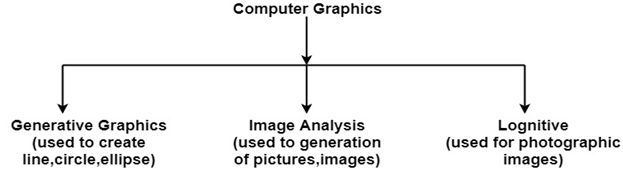
\includegraphics{cg}
\caption{Computer Graphics}
\end{figure}
\section*{Defination}

It is the use of computers to create and manipulate pictures on a display device. It comprises of software techniques to create, store, modify, represents pictures.
 \cleardoublepage
  
  %table of contents
  \tableofcontents
  \thispagestyle{empty}
  \cleardoublepage
  
  %main body stuff
  \pagenumbering{arabic}
  \setcounter{page}{1}  
  
  \section{Cathode Ray Tube}
 The primary output device in a graphical system is the video monitor. The main element of a video monitor is the Cathode Ray Tube CRT, shown in the following illustration.

The operation of CRT is very simple 
 \begin{itemize}
  \item The electron gun emits a beam of electrons cathoderays.
  \item The electron beam passes through focusing and deflection systems that direct it towards specified positions on the phosphor-coated screen.
  \item When the beam hits the screen, the phosphor emits a small spot of light at each position contacted by the electron beam.
  \item It redraws the picture by directing the electron beam back over the same screen points quickly.
\end{itemize}
\begin{figure}[h]
\centering
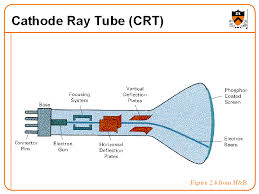
\includegraphics{crt2}
\caption{Cathode Ray Tube}
\end{figure}

 \section{Application of Computer Graphics}
 Computer Graphics has numerous applications, some of which are listed below 


  \begin{itemize}
    \item Computer graphics user interfaces GUIs  A graphic, mouse-oriented paradigm which allows the user to interact with a computer.
    \item Business presentation graphics  "A picture is worth a thousand words".
    \item  Cartography Drawing maps.
    \item Weather Maps  Real-time mapping, symbolic representations.
    \item Satellite Imaging  Geodesic images.
    \item Photo Enhancement  Sharpening blurred photos.
    
  \end{itemize}
  \begin{figure}[h]
  \centering
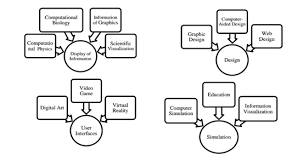
\includegraphics{ap}
\caption{Application of Computer Graphics}
\end{figure}

  \newpage
  \section{Raster Scan}
In a raster scan system, the electron beam is swept across the screen, one row at a time from top to bottom. As the electron beam moves across each row, the beam intensity is turned on and off to create a pattern of illuminated spots.

Picture definition is stored in memory area called the Refresh Buffer or Frame Buffer. This memory area holds the set of intensity values for all the screen points. Stored intensity values are then retrieved from the refresh buffer and “painted” on the screen one row scanline at a time as shown in the following illustration.

Each screen point is referred to as a pixel pictureelement or pel. At the end of each scan line, the electron beam returns to the left side of the screen to begin displaying the next scan line.


 
 \begin{figure}[h]
 \centering
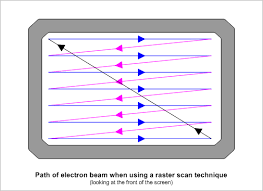
\includegraphics{rs}
\caption{Raster Scan}
\end{figure}
 
  \section{Bresenham’s Line Generation}
The Bresenham algorithm is another incremental scan conversion algorithm. The big advantage of this algorithm is that, it uses only integer calculations. Moving across the x axis in unit intervals and at each step choose between two different y coordinates.
 
   \newpage
  \section{Image types}
  \subsection{Two-dimensional}

Raster graphic sprites (left) and masks (right)
2D computer graphics are the computer-based generation of digital images—mostly from models, such as digital image, and by techniques specific to them.

2D computer graphics are mainly used in applications that were originally developed upon traditional printing and drawing technologies such as typography. In those applications, the two-dimensional image is not just a representation of a real-world object, but an independent artifact with added semantic value; two-dimensional models are therefore preferred because they give more direct control of the image than 3D computer graphics, whose approach is more akin to photography than to typography.
  \subsection{Pixel art}
  
 A large form of digital art, pixel art is created through the use of raster graphics software, where images are edited on the pixel level. Graphics in most old (or relatively limited) computer and video games, graphing calculator games, and many mobile phone games are mostly pixel art.
 \subsection{Sprite graphics}
 
 A sprite is a two-dimensional image or animation that is integrated into a larger scene. Initially including just graphical objects handled separately from the memory bitmap of a video display, this now includes various manners of graphical overlays.

Originally, sprites were a method of integrating unrelated bitmaps so that they appeared to be part of the normal bitmap on a screen, such as creating an animated character that can be moved on a screen without altering the data defining the overall screen. Such sprites can be created by either electronic circuitry or software. In circuitry, a hardware sprite is a hardware construct that employs custom DMA channels to integrate visual elements with the main screen in that it super-imposes two discrete video sources. Software can simulate this through specialized rendering methods.

  \newpage
  
  \subsection{Vector graphics}
 Vector graphics formats are complementary to raster graphics. Raster graphics is the representation of images as an array of pixels and is typically used for the representation of photographic images.[26] Vector graphics consists in encoding information about shapes and colors that comprise the image, which can allow for more flexibility in rendering. There are instances when working with vector tools and formats is best practice, and instances when working with raster tools and formats is best practice. There are times when both formats come together. An understanding of the advantages and limitations of each technology and the relationship between them is most likely to result in efficient and effective use of tools.


\subsection{Three-dimensional}
 
 3D graphics, compared to 2D graphics, are graphics that use a three-dimensional representation of geometric data. For the purpose of performance, this is stored in the computer. This includes images that may be for later display or for real-time viewing.

Despite these differences, 3D computer graphics rely on similar algorithms as 2D computer graphics do in the frame and raster graphics (like in 2D) in the final rendered display. In computer graphics software, the distinction between 2D and 3D is occasionally blurred; 2D applications may use 3D techniques to achieve effects such as lighting, and primarily 3D may use 2D rendering techniques.

3D computer graphics are the same as 3D models. The model is contained within the graphical data file, apart from the rendering. However, there are differences that include the 3D model is the representation of any 3D object. Until visually displayed a model is not graphic. Due to printing, 3D models are not only confined to virtual space. 3D rendering is how a model can be displayed. Also can be used in non-graphical computer simulations and calculations.

\subsection{Computer animation}

Computer animation is the art of creating moving images via the use of computers. It is a subfield of computer graphics and animation. Increasingly it is created by means of 3D computer graphics, though 2D computer graphics are still widely used for stylistic, low bandwidth, and faster real-time rendering needs. Sometimes the target of the animation is the computer itself, but sometimes the target is another medium, such as film. It is also referred to as CGI (Computer-generated imagery or computer-generated imaging), especially when used in films.

Virtual entities may contain and be controlled by assorted attributes, such as transform values (location, orientation, and scale) stored in an object's transformation matrix. Animation is the change of an attribute over time. Multiple methods of achieving animation exist; the rudimentary form is based on the creation and editing of keyframes, each storing a value at a given time, per attribute to be animated. The 2D/3D graphics software will change with each keyframe, creating an editable curve of a value mapped over time, in which results in animation. Other methods of animation include procedural and expression-based techniques: the former consolidates related elements of animated entities into sets of attributes, useful for creating particle effects and crowd simulations; the latter allows an evaluated result returned from a user-defined logical expression, coupled with mathematics, to automate animation in a predictable way (convenient for controlling bone behavior beyond what a hierarchy offers in skeletal system set up).

To create the illusion of movement, an image is displayed on the computer screen then quickly replaced by a new image that is similar to the previous image, but shifted slightly. This technique is identical to the illusion of movement in television and motion pictures.
   \newpage
 \section{Concepts and principles}
Images are typically created by devices such as cameras, mirrors, lenses, telescopes, microscopes, etc.

Digital images include both vector images and raster images, but raster images are more commonly used.
  \subsection{Pixel}
  In digital imaging, a pixel (or picture element[27]) is a single point in a raster image. Pixels are placed on a regular 2-dimensional grid, and are often represented using dots or squares. Each pixel is a sample of an original image, where more samples typically provide a more accurate representation of the original. The intensity of each pixel is variable; in color systems, each pixel has typically three components such as red, green, and blue.

Graphics are visual presentations on a surface, such as a computer screen. Examples are photographs, drawing, graphics designs, maps, engineering drawings, or other images. Graphics often combine text and illustration. Graphic design may consist of the deliberate selection, creation, or arrangement of typography alone, as in a brochure, flier, poster, web site, or book without any other element. Clarity or effective communication may be the objective, association with other cultural elements may be sought, or merely, the creation of a distinctive style.
\subsection{Primitives}

Primitives are basic units which a graphics system may combine to create more complex images or models.Examples would be sprites and character maps in 2d video games, geometric primitives in CAD, or polygons or triangles in 3d rendering. Primitives may be supported in hardware for efficient rendering, or the building blocks provided by a graphics application.
\subsection{Rendering}
Rendering is the generation of a 2D image from a 3D model by means of computer programs. A scene file contains objects in a strictly defined language or data structure; it would contain geometry, viewpoint, texture, lighting, and shading information as a description of the virtual scene. The data contained in the scene file is then passed to a rendering program to be processed and output to a digital image or raster graphics image file. The rendering program is usually built into the computer graphics software, though others are available as plug-ins or entirely separate programs. The term "rendering" may be by analogy with an "artist's rendering" of a scene. Although the technical details of rendering methods vary, the general challenges to overcome in producing a 2D image from a 3D representation stored in a scene file are outlined as the graphics pipeline along a rendering device, such as a GPU. A GPU is a device able to assist the CPU in calculations. If a scene is to look relatively realistic and predictable under virtual lighting, the rendering software should solve the rendering equation. The rendering equation does not account for all lighting phenomena, but is a general lighting model for computer-generated imagery. 'Rendering' is also used to describe the process of calculating effects in a video editing file to produce final video output.

3D projection
3D projection is a method of mapping three dimensional points to a two dimensional plane. As most current methods for displaying graphical data are based on planar two dimensional media, the use of this type of projection is widespread, especially in computer graphics, engineering and drafting.
  \newpage
  \subsection{Ray tracing}
  Ray tracing is a technique for generating an image by tracing the path of light through pixels in an image plane. The technique is capable of producing a very high degree of photorealism; usually higher than that of typical scanline rendering methods, but at a greater computational cost.
 
 \subsection{Shading}
 Shading refers to depicting depth in 3D models or illustrations by varying levels of darkness. It is a process used in drawing for depicting levels of darkness on paper by applying media more densely or with a darker shade for darker areas, and less densely or with a lighter shade for lighter areas. There are various techniques of shading including cross hatching where perpendicular lines of varying closeness are drawn in a grid pattern to shade an area. The closer the lines are together, the darker the area appears. Likewise, the farther apart the lines are, the lighter the area appears. The term has been recently generalized to mean that shaders are applied.
 
\subsection{Texture mapping}
Texture mapping is a method for adding detail, surface texture, or colour to a computer-generated graphic or 3D model. Its application to 3D graphics was pioneered by Dr Edwin Catmull in 1974. A texture map is applied (mapped) to the surface of a shape, or polygon. This process is akin to applying patterned paper to a plain white box. Multitexturing is the use of more than one texture at a time on a polygon.[28] Procedural textures (created from adjusting parameters of an underlying algorithm that produces an output texture), and bitmap textures (created in an image editing application or imported from a digital camera) are, generally speaking, common methods of implementing texture definition on 3D models in computer graphics software, while intended placement of textures onto a model's surface often requires a technique known as UV mapping (arbitrary, manual layout of texture coordinates) for polygon surfaces, while non-uniform rational B-spline (NURB) surfaces have their own intrinsic parameterization used as texture coordinates. Texture mapping as a discipline also encompasses techniques for creating normal maps and bump maps that correspond to a texture to simulate height and specular maps to help simulate shine and light reflections, as well as environment mapping to simulate mirror-like reflectivity, also called gloss.
\newpage
 \section{Pioneers in computer graphics}
 \subsection{Charles Csuri}
  Charles Csuri is a pioneer in computer animation and digital fine art and created the first computer art in 1964. Csuri was recognized by Smithsonian as the father of digital art and computer animation, and as a pioneer of computer animation by the Museum of Modern Art (MoMA) and Association for Computing Machinery-SIGGRAPH.
  
  \subsection{Donald P. Greenberg}
  Donald P. Greenberg is a leading innovator in computer graphics. Greenberg has authored hundreds of articles and served as a teacher and mentor to many prominent computer graphic artists, animators, and researchers such as Robert L. Cook, Marc Levoy, Brian A. Barsky, and Wayne Lytle. Many of his former students have won Academy Awards for technical achievements and several have won the SIGGRAPH Achievement Award. Greenberg was the founding director of the NSF Center for Computer Graphics and Scientific Visualization.
  \subsection{Other pioneers}
  \begin{itemize}
  \item Pierre Bézier
  \item Jim Blinn
   \item Jack Bresenham
    \item John Carmack
    \item Paul de Casteljau
    \item Ed Catmull
    \item Frank Crow
    \item James D. Foley
  \end{itemize}
  \subsection{Organizations}
  \begin{itemize}
  \item SIGGRAPH
   \item Bell Telephone Laboratories
    \item United States Armed Forces, particularly the Whirlwind computer and SAGE Project
     \item The computer science department of the University of Utah
     
  \end{itemize}
  
  
  \newpage
  \section{Study of computer graphics}
  The study of computer graphics is a sub-field of computer science which studies methods for digitally synthesizing and manipulating visual content. Although the term often refers to three-dimensional computer graphics, it also encompasses two-dimensional graphics and image processing.

As an academic discipline, computer graphics studies the manipulation of visual and geometric information using computational techniques. It focuses on the mathematical and computational foundations of image generation and processing rather than purely aesthetic issues. Computer graphics is often differentiated from the field of visualization, although the two fields have many similarities.
\begin{figure}[h]
\centering
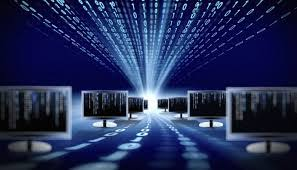
\includegraphics{sg}
\end{figure}
Computer graphics will continue to get more sophisticated. Their 3-D photorealistic capabilities and ability to predict changes over time have revolutionized product development and marketing, as well as scientific research and education. They are responsible for superior special effects in movies and on television. Many newspapers and magazines use only computer-generated graphics. They add an aesthetic and emotional dimension to text. Computer graphics affect everyone's life in almost every aspect every day.
 

\end{document}